\chapter{Background}
% TODO


\section{Positioning in the distributed Test Support System}
% TODO


\section{TCP/IP Reference Model}

Protocols are the basis for communication between instances in a network. They specify rules that must be followed by all communication partners \cite{Tanenbaum2010}. Reference models arrange protocols hierarchically in layers. Each layer solves a specific part of the communication task and uses the services of the layer below while providing certain services to the layer above \cite{Weigel2021}.

\begin{figure}
    \centering
    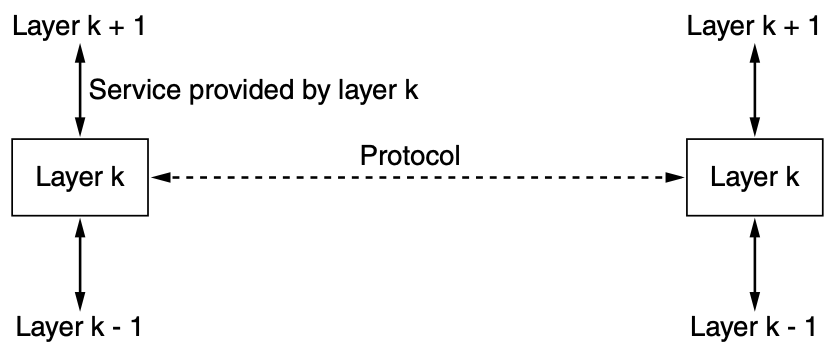
\includegraphics[width=0.7\linewidth]{figures/tcpip_refmodel/image1.png}
    \caption[Relationship between service and protocol]{Relationship between service and protocol. Source: \cite{Tanenbaum2010}.}
    \label{fig:ServiceProtRelation}
\end{figure}

Figure \ref{fig:ServiceProtRelation} illustrates the relationship between service and protocol. A service refers to a set of operations that a layer provides to the layer above it, and it defines the interface between the two layers \cite{Tanenbaum2010}.

A protocol is a set of rules that define the format of messages exchanged within a layer \cite{Tanenbaum2010}. These rules define the implementation of the service offered by the layer The transparency principle applies, meaning that the implementing protocol is transparent to the service user and can be changed as long as the service offered remains unchanged \cite{Weigel2021}.

\begin{figure}[h!]
    \centering
    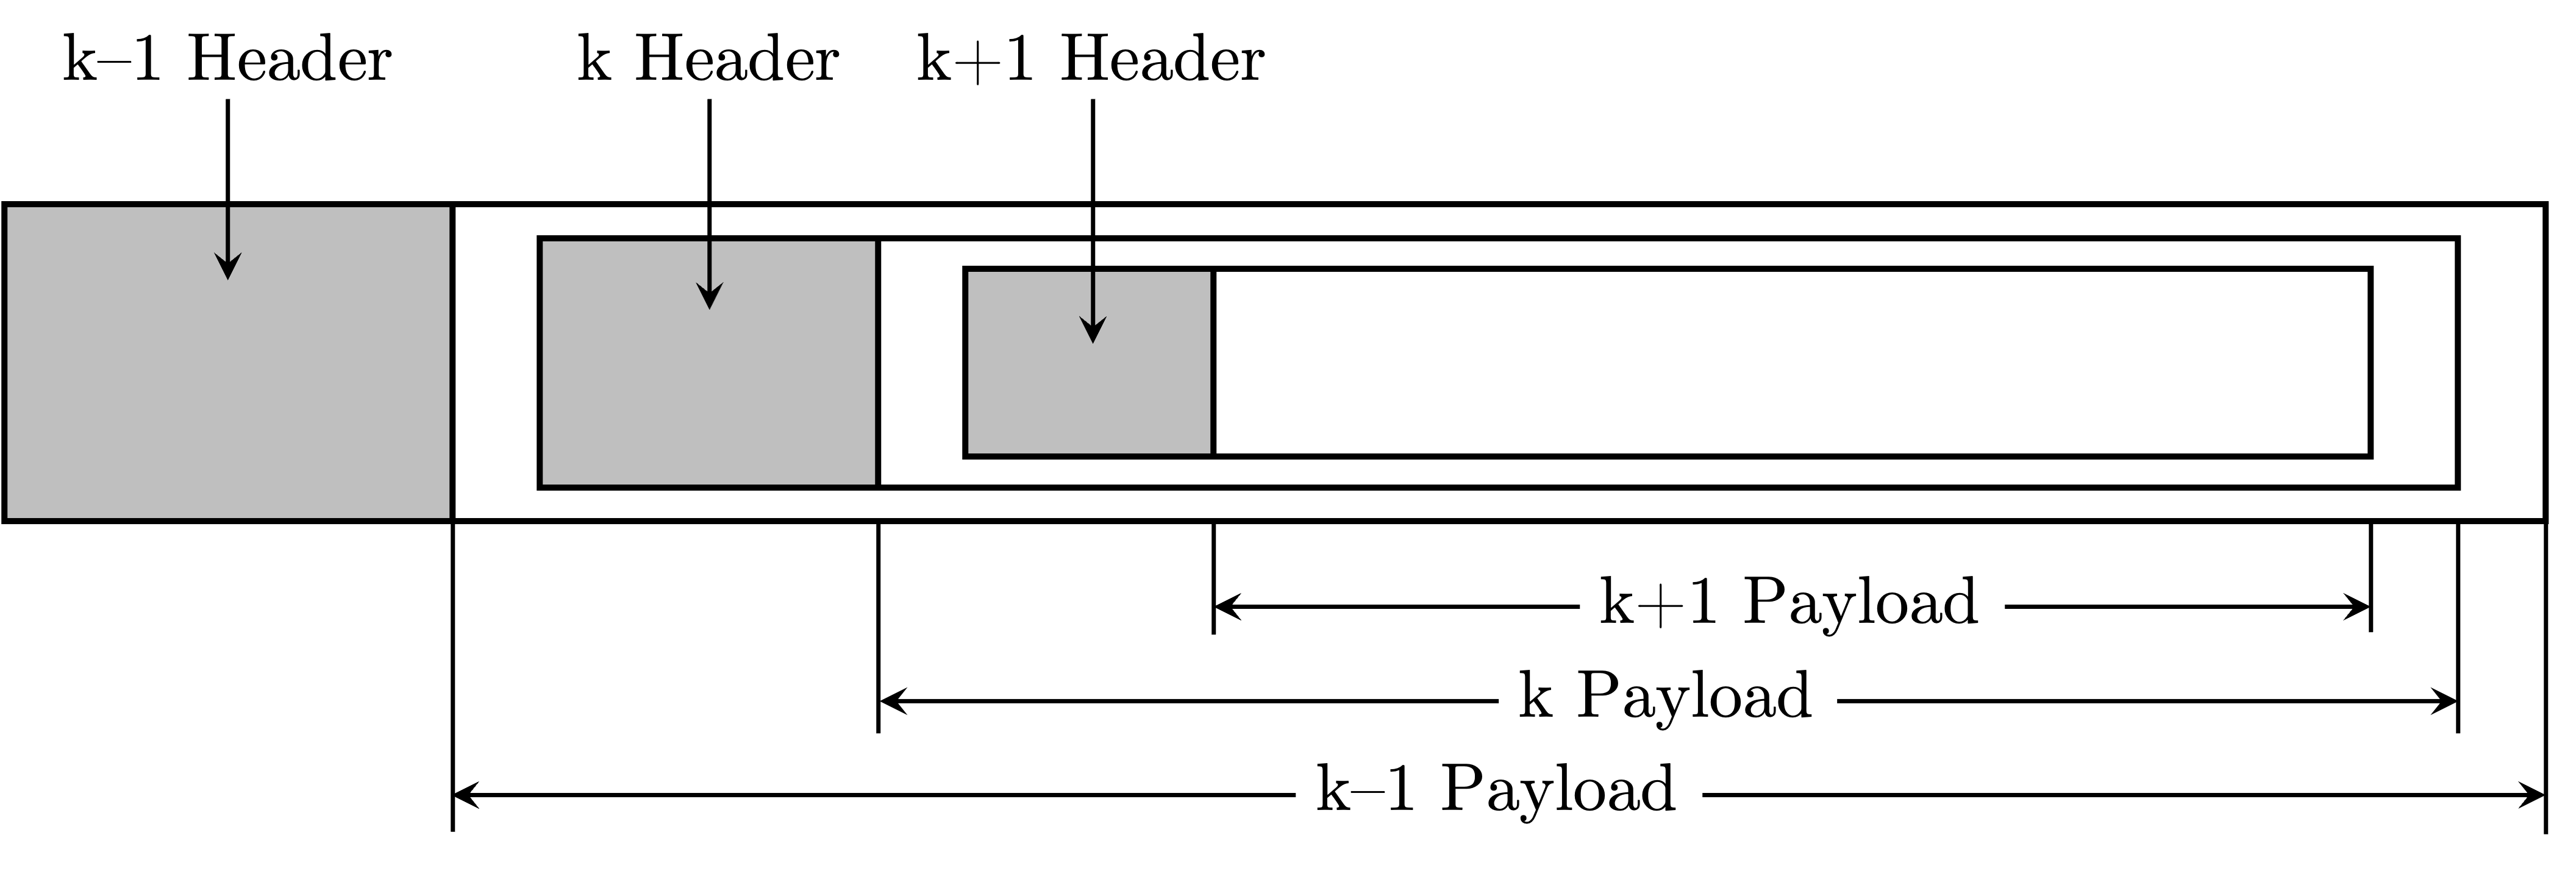
\includegraphics[width=1\linewidth]{figures/tcpip_refmodel/image2.png}
    \caption[Encapsulation Principle]{Encapsulation Principle. Adapted from: \cite{Tanenbaum2010}.}
    \label{fig:EncapsulationPrinciple}
\end{figure}

Protocols define the format of control information required by layer k to provide the service. This information is attached as a header or trailer to the data of layer k + 1, known as the payload, and is removed by the receiving instance. This principle is known as the 'Encapsulation Principle' and is illustrated in Figure \ref{fig:EncapsulationPrinciple} \cite{Tanenbaum2010}.



\subsection{Introduction of the Reference Model}

The following section presents a explanation of the TCP/IP reference model. Throughout this section, we will refer to the hybrid reference model proposed by Andrew S. Tanenbaum in \cite{Tanenbaum2010}. Figure \ref{fig:RefModel} shows this hybrid reference model. The physical layer is at the bottom, and the application layer is at the top. The tasks of each layer are briefly described here. For additional information, please refer to \cite{Tanenbaum2010}.

\begin{figure}[h]
    \centering
    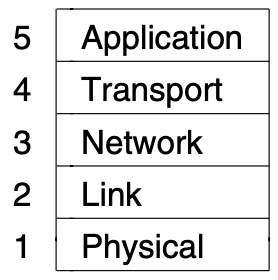
\includegraphics[width=0.25\linewidth]{figures/tcpip_refmodel/image3.png}
    \caption[Hybrid TCP/IP Reference Model]{Hybrid TCP/IP Reference Model. Source: \cite{Tanenbaum2010}.}
    \label{fig:RefModel}
\end{figure}
	
	
\begin{itemize}
\item The \textbf{Physical Layer} serves as the interface between a network node and the transmission medium, responsible for transmitting a bit stream. This involves line coding, which converts binary data into a signal. Additionally, the physical layer encompasses the transmission medium and the connection to this medium \cite{Tanenbaum2010, Weigel2021}.
\item The \textbf{Link Layer} facilitates reliable transmission of a sequence of bits (called a frame) between adjacent network nodes. This encompasses frame synchronization, which involves detecting frame boundaries in the bit stream, error protection, flow control, channel access control, and addressing \cite{Weigel2021}.
\item The \textbf{Network Layer} provides end-to-end communication between two network nodes. This includes addressing and routing \cite{Tanenbaum2010, Weigel2021}.
\item The \textbf{Transport Layer} provides the transfer of a data stream of any length between two application processes. This involves collecting outgoing messages from all application processes and distributing incoming messages to them \cite{Weigel2021}.
\item The \textbf{Application Layer} serves as the interface to the application. It is responsible for implementing protocols for network use, such as file transfer or network management \cite{Weigel2021}.
\end{itemize}



\subsection{Protocols of the Reference Model}

\begin{figure}[h]
    \centering
    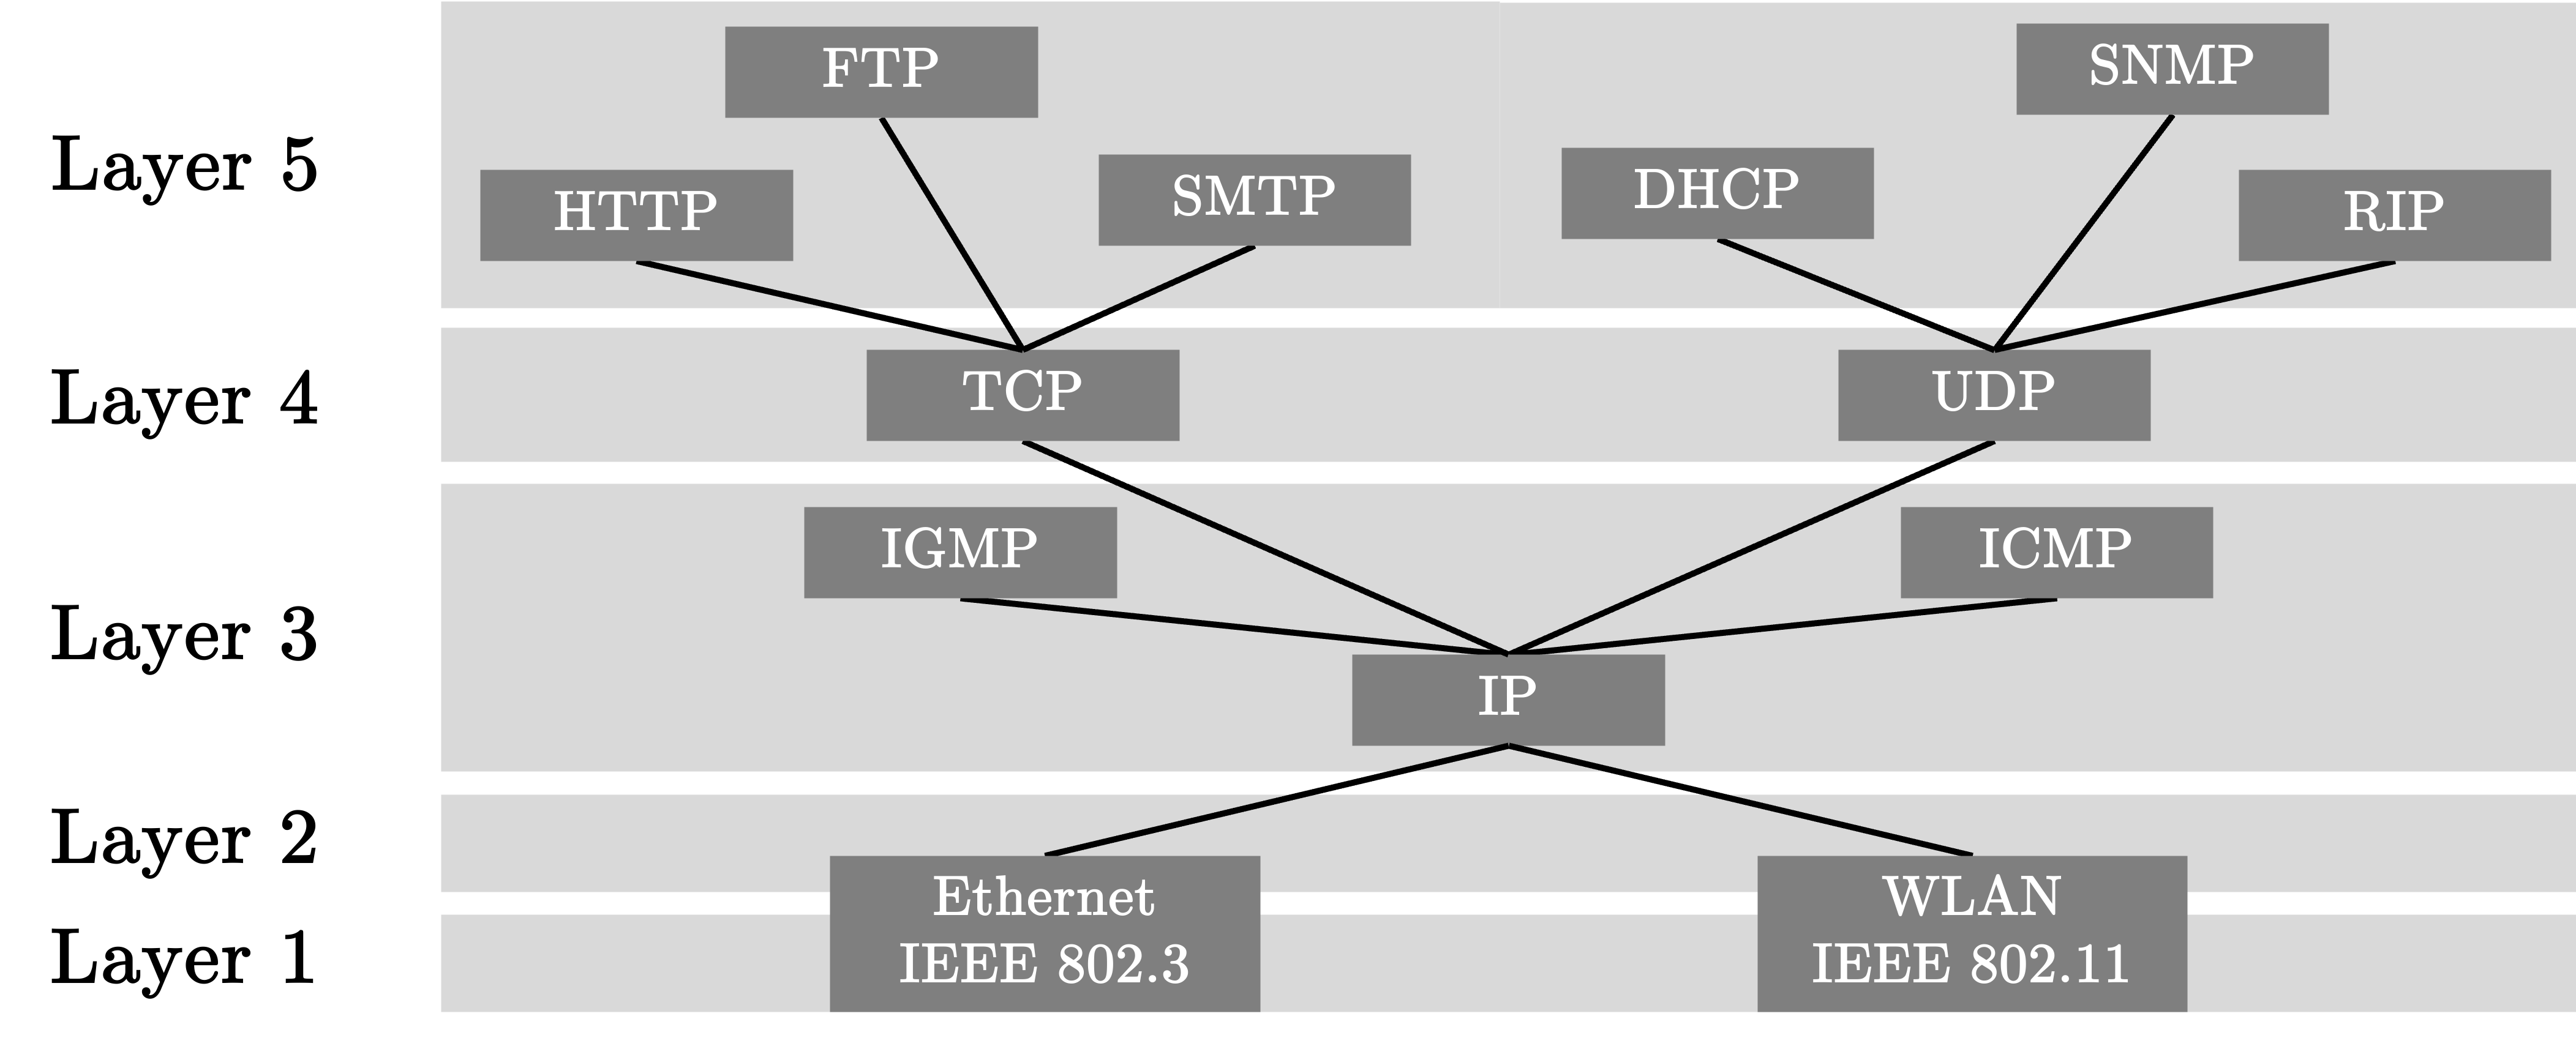
\includegraphics[width=1\linewidth]{figures/tcpip_refmodel/image4.png}
    \caption[Selection of important protocols of the hybrid TCP/IP Reference Model]{Selection of important protocols of the hybrid TCP/IP Reference Model. Adapted from: \cite{Weigel2021}.}
    \label{fig:RefModelProtos}
\end{figure}

Figure \ref{fig:RefModelProtos} shows a selection of important protocols of the TCP/IP reference model including their assignment to the respective layer. The illustration also shows the dependency of the protocols on each other.

In this section, the characteristics of the protocols TCP, UDP, IP and Ethernet (IEEE 802.3), which are relevant for this work, are explained in detail according to \cite{Tanenbaum2010}. Further information about the protocols of the TCP/IP reference model can be found in \cite{Tanenbaum2010}.


\subsubsection{Ethernet (IEEE 802.3)}
Ethernet, as defined by IEEE standard 802.3, specifies both hardware and software for wired data networks.  This means that Ethernet includes both the physical layer and the link layer of the presented hybrid TCP/IP reference model.


\paragraph{Ethernet Physical Layer}
The Ethernet physical layer consists of a number of standards that define different media types associated with different transmission rates and cable lengths. 

Ethernet defines physical layer standards with transmission rates ranging from 10 Mbit/s to 1.6 Tbit/s, which is currently under development as the 802.3dj standard \cite{IEEEOpeningPlenary}. Both fiber and copper are used as transmission media. In the following, the 802.3an standard will be briefly discussed, since it is the one that will be used most in this thesis.

The 802.3an standard was published in 2006 and defines data transmission with a transmission rate of 10 Gbit/s over twisted-pair cables \cite{10GigabitEthernet}, also referred to as 10 GbE. Twisted-pair cables are copper cables in which pairs of copper wires are twisted together to reduce electromagnetic interference. Twisted-pair cables are divided into categories based on various characteristics, such as shielding or twist strength \cite{isoiec11801}. For 802.3an, a maximum cable length of 100 meters is specified in conjunction with Cat7 cables. 802.3an specifies the RJ45 connector as the plug connector.

According to 802.3an, the PAM16 line coding is used for Ethernet at 10 Gbps. It uses the principle of pulse amplitude modulation, which is described in detail in \cite{PulseAmplitudeModulation}. PAM16 allows the transmission of data by varying the amplitude of a signal in 16 different stages. Each stage represents four bits of information.

In addition to 802.3an, the Ethernet physical layer according to 802.3ae was also used in this work. This also defines the physical layer with a transmission rate of 10 Gbit/s. However, fiber optic cables are used in conjunction with transceiver modules called SPF+ SR \cite{10GigabitEthernet}.

\paragraph{Ethernet Link Layer} \label{chap:EthLinkLayer}
At the link layer, Ethernet defines frame formatting, addressing, error detection, and access control. This is also called the Medium Access Control (MAC) sublayer.

\begin{figure}[h]
    \centering
    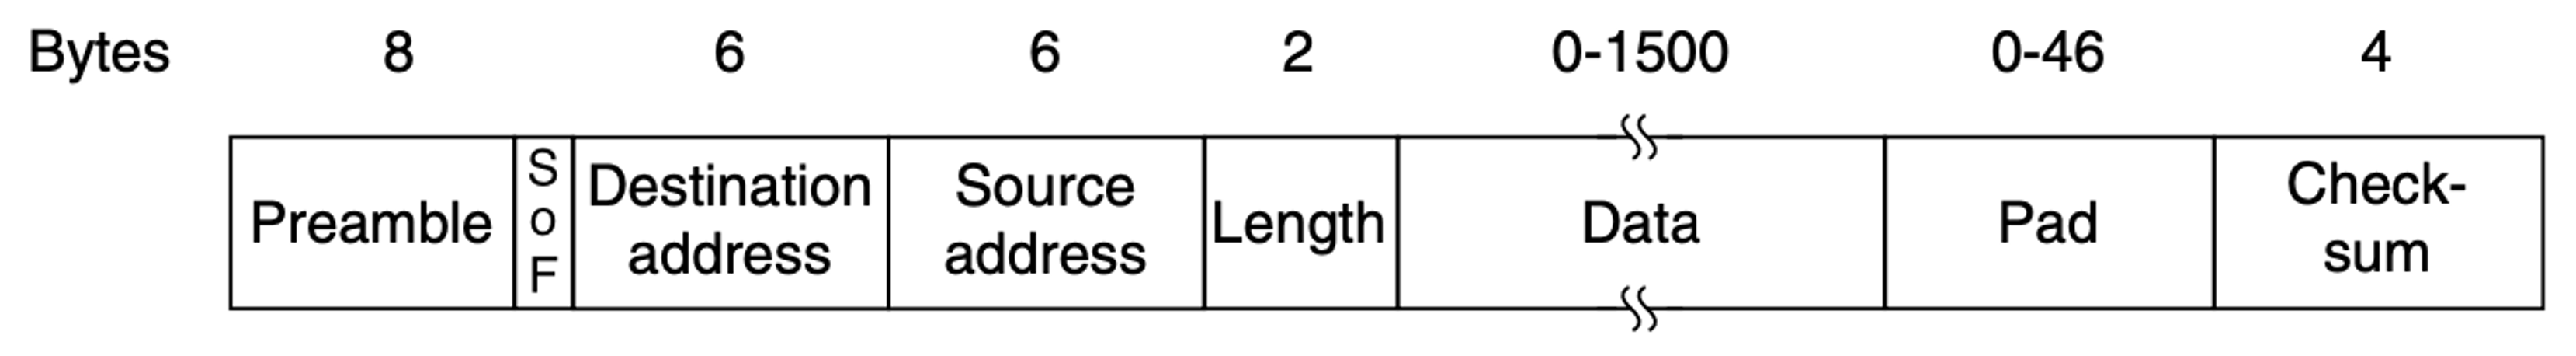
\includegraphics[width=1\linewidth]{figures/tcpip_refmodel/image5.png}
    \caption[Structure of the Ethernet frame]{Structure of the Ethernet frame. Source: \cite{Tanenbaum2010}.}
    \label{fig:EthernetFrame}
\end{figure}

Figure \ref{fig:EthernetFrame} shows the IEE 802.3 frame format. The Ethernet header consists of the fields '\textit{Destination address}', '\textit{Source address}' and '\textit{Length}' and therefore has a size of 14 bytes.

Each frame begins with a \textit{preamble}. This has a length of 8 bytes and contains the bit sequence 10101010. An exception is the last byte, which contains the bit sequence 10101011 and is referred to as the \textit{Start of Frame} (SoF). The preamble is used for synchronization between the sender and receiver. The last byte of the preamble marks the start of a frame \cite{Tanenbaum2010}.

This is followed by the \textit{destination} and \textit{source address}. This is the MAC address, which is uniquely assigned globally to a network interface \cite{Weigel2021}. This consists of a manufacturer code with a length of 3 bytes, followed by the serial number of the network interface, which also has a length of 3 bytes. The MAC address enables the Ethernet protocol to uniquely identify a station in the local network.

The \textit{Length} field specifies the length of the next data field. In IEEE 802.3 Ethernet, this has a maximum length, called the Maximum Transfer Unit (MTU), of 1500 bytes. However, there are Ethernet implementations that use a larger MTU than specified in the original standard. These are known as jumbo frames \cite{EthernetJumboFrames2009}.

In addition to a maximum length, the Ethernet standard also specifies a minimum length. An entire Ethernet frame must therefore have a minimum length of 64 bytes from the destination address to the checksum. To ensure that this can be achieved even with a small data field, padding information is added. The specification of the minimum length is related to the access control used.

The Ethernet frame ends with a 4-byte \textit{checksum} that is used for the Cyclic Redundancy Check (CRC) based on polynomial divisions, as explained in \cite{Tanenbaum2010}.  This checksum serves to detect errors during transmission.

Ethernet originally used a shared transmission medium, allowing multiple communication participants to use it simultaneously. To control access, the MAC sublayer employs the CSMA/CD algorithm, ensuring that only one device transmits data at a time. Each device listens to the medium (carrier sense) before sending data to determine whether it is free. It also performs collision detection to determine whether two devices have started sending at the same time. In such a case, the devices stop the transmission and retry it after a random waiting time to avoid the collision \cite{Tanenbaum2010}.

The 802.3an specification for 10 Gigabit Ethernet is exclusively for point-to-point full-duplex connections, which eliminates the need for access control such as CSMA/CD. As a result, it is no longer included in the specification \cite{10GbEDefinition}.

In order to connect multiple network devices with point-to-point connections, Ethernet switches are used. They have multiple ports and forward packets based on the MAC address. Ethernet switches operate on layer 2 of the reference model.

To summarise, with Ethernet there is no guarantee that data will be transmitted reliably and without loss. Although Ethernet uses CRC for error detection, faulty frames are generally discarded. Additionally, Ethernet does not provide flow control or overload detection, which must be performed by a higher layer.


\subsubsection{IP}

The Internet Protocol (IP) is a central protocol in the TCP/IP reference model. Its tasks include connecting different networks, addressing network participants, and fragmenting packets \cite{Weigel2021}. IP is a connectionless protocol that operates on the 'best effort' principle, meaning it does not guarantee delivery.

There are two versions of the Internet Protocol: IPv4 and IPv6. As this work uses the IPv4 protocol, it is presented in more detail below.

\paragraph{IP Header}

The IPv4 datagram is divided into a header and a payload. The header typically spans 20 bytes, but may also include an optional variable-length section. The header is shown in Figure \ref{fig:IPHeader}.

\begin{figure}[h]
    \centering
    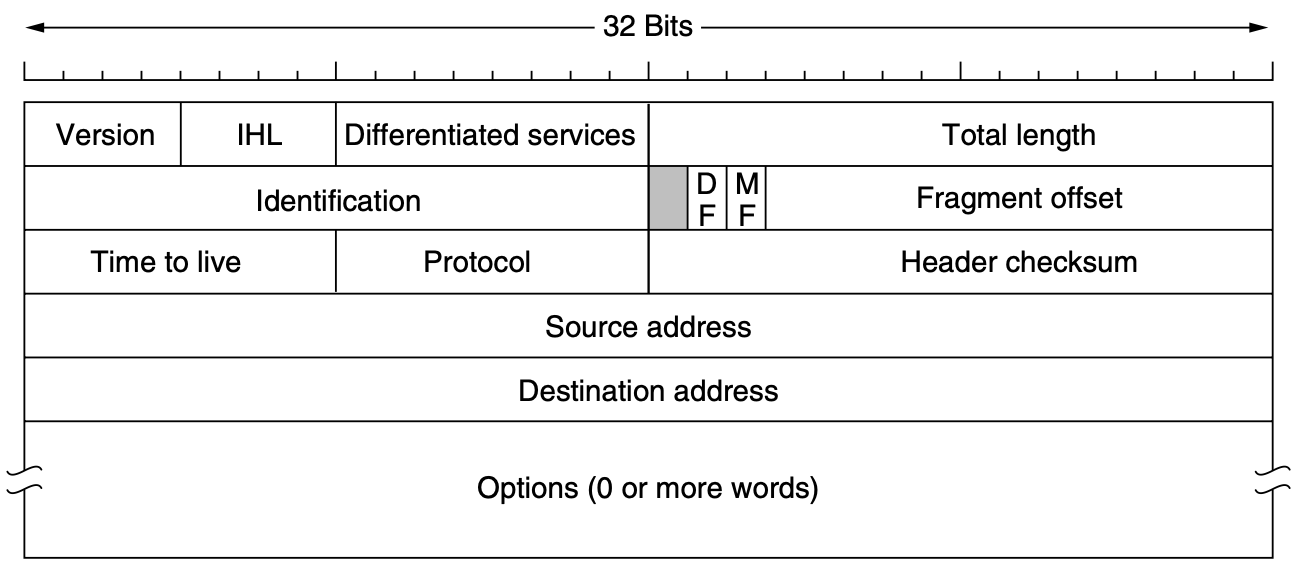
\includegraphics[width=1\linewidth]{figures/tcpip_refmodel/image7.png}
    \caption[Structure of the IP Header]{Structure of the IP Header. Source: \cite{Tanenbaum2010}.}
    \label{fig:IPHeader}
\end{figure}

The first field in the header is the 4-bit \textit{Version} field. This indicates the IP version used. For IPv4, the value is always 4.

The \textit{IHL} (Internet Header Length) field specifies the number of 32-bit words in the header. This is necessary because the header can contain options and therefore has a variable length. The minimum value of the field is 5 if there are no options.

The \textit{Differenciated Services} field specifies the service class of a packet, allowing for prioritisation of certain data traffic using Quality of Service (QoS). For a more detailed description of Quality of Service, please refer to section \ref{background:tuning:qualityofservice}.

The \textit{Total Length} field indicates the total length of the datagram, including the header. Due to the field size of 16 bits, the maximum length is 65535 bytes. However, a packet's length is also limited by the Layer 2 MTU \cite{Weigel2021}, resulting in datagrams being split into multiple packets, known as fragmentation. 

The \textit{Identification} field is assigned a number by the sender, which is shared by all fragments of a datagram.

A flag field with a length of 3 bits follows, with the first bit being unused. The second section includes the 'Don't Fragment' (\textit{DF}) flag, which indicates that intermediate stations should not fragment this packet. The third section contains the 'More Fragments' (\textit{MF}) flag, which indicates whether additional fragments follow. This flag is set for all fragments except the last one of a datagram.

The \textit{Fragment Offset} field specifies the position of a fragment in the entire datagram.

The \textit{Time to live} (TTL) field specifies the maximum lifetime of a packet. The TTL value is measured in seconds and can be set to a maximum of 255 seconds. This is done to prevent packets from endlessly circulating in the network.

The \textit{Protocol} field identifies the Layer 4 protocol used for the service. This allows the network layer to forward the packet to the corresponding protocol of the transport layer. The numbering of the protocols is standardized throughout the Internet.

The \textit{Header checksum} field contains the checksum of the fields in the IP header. The IP datagram's user data is not verified for efficiency reasons \cite{Holtkamp2024Internet}. The checksum is calculated by taking the 1's complement of the sum of all 16-bit half-words in the header. It is assumed that the checksum is zero at the start of the calculation for the purpose of this algorithm.

The two 32-bit fields \textit{Source Address} and \textit{Destination Address} contain the Internet Protocol address, called the IP address. Section \ref{chap:IPandRouting} provides further details on this topic.

The \textit{Options} field can be used to add additional information to the IP protocol. For example, there are options to mark the route of a packet.


\paragraph{IP addresses and routing} \label{chap:IPandRouting}

This section provides a brief description of the structure and important properties of IP addresses. The network examined in this thesis is an isolated local network that is not connected to other networks. As a result, the network layer does not perform any routing based on IP addresses. For further information on routing, please refer to \cite{Tanenbaum2010}.

\begin{figure}[h]
    \centering
    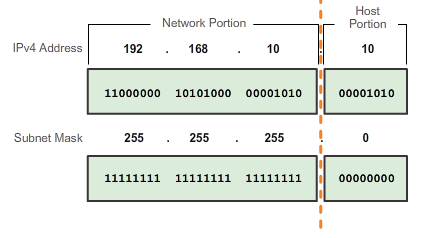
\includegraphics[width=0.8\linewidth]{figures/tcpip_refmodel/image8.png}
    \caption[Structure of the IP address and subnet mask]{Structure of the IP address and subnet mask. Source: \cite{CSE252ImageSubnet}.}
    \label{fig:IPSubnet}
\end{figure}

Every participant on the Internet has a unique address, known as an IP address. This has a total length of 32 bits and a hierarchical structure that divides the IP address into a network portion and a host portion. The division between the two parts is variable and is defined by a so-called subnet mask, which is illustrated in Figure \ref{fig:IPSubnet}. The bits of the network portion of the IP address are marked with ones.

\begin{itemize}
\item The \textbf{network portion} identifies a specific network, such as a local Ethernet network, and is the same for all participants in this network.
\item The \textbf{host portion} identifies a specific device within this network.
\end{itemize}

Routing, which is another important task of the network layer, is based on IP addresses. The packet can be directed to its destination using the network portion of the IP address. The path to the destination is determined by specific routing algorithms. As mentioned earlier, the thesis only considers an isolated local network, so further discussion on routing will be omitted.


\paragraph{Address Resolution Protocol}

The Address Resolution Protocol, abbreviated to ARP, is an auxiliary protocol of the network layer. Its task is to map the IP addresses to a MAC address and vice versa, as the sending and receiving of data in the underlying link layer is based on these MAC addresses \cite{Weigel2021}.


\paragraph{Fragmentation and Defragmentation}

As explained in \ref{chap:EthLinkLayer}, the link layer defines a maximum data size known as MTU. Since IPv4 datagrams have a maximum size of 65535 bytes, they must be divided into smaller packets, or fragments, each with its own IP header.

The IP header (refer to Figure \ref{fig:IPHeader}) contains information necessary for the target system to assemble fragmented packets, a process known as defragmentation. This includes the ID that assigns all fragmented packets to a datagram, as well as the fragment offset that specifies their position within the datagram. The 'More Fragment' flag indicates whether additional fragments will follow.

Fragmentation has the advantage of allowing IPv4 datagrams larger than the MTU to be sent, but the disadvantage is that the loss of a single fragment results in the loss of the entire datagram. Additionally, fragmentation can cause packet reordering \cite{IPFragDetail}.

\subsubsection{TCP and UDP}
TPC and UDP are transport layer protocols. As a service, they provide the transmission of a data stream of any length between two application processes. The services of the network layer are used for this purpose.

\paragraph{TCP}

TCP provides \textbf{reliable} transmission of a byte stream in a \textbf{connection-oriented} manner. A virtual connection is established between the two instances before transmission, which is terminated after transmission.

TCP also implements flow control to ensure reliable data transfer between sender and receiver without losses and to prevent overloading at the receiver.  TCP provides congestion control to prevent network overload and ensures reliable transmission using Positive Acknowledgement with Re-Transmission (PAR) algorithm \cite{Holtkamp2024Transport}.  

TCP is known for its secure data transmission. However, it requires a significant amount of control information to implement its functions. The Transmission Control Protocol (TCP) header is 20 bytes in size. In addition to an application identifier (port number), it contains flow control and congestion control information. This overhead can negatively impact transmission speed. Additionally, the data loss from the underlying layers combined with the flow control used by TCP leads to delays and reduced throughput, which can have a significant impact on the performance of the application.

\paragraph{UDP}

In contrast to TCP, UDP is an \textbf{unreliable} and \textbf{connectionless} protocol. The protocol sends packets, called datagrams or segments, individually. UDP lacks mechanisms for detecting the loss of individual datagrams, and the correct sequence of these is not guaranteed.

\begin{figure}[h]
    \centering
    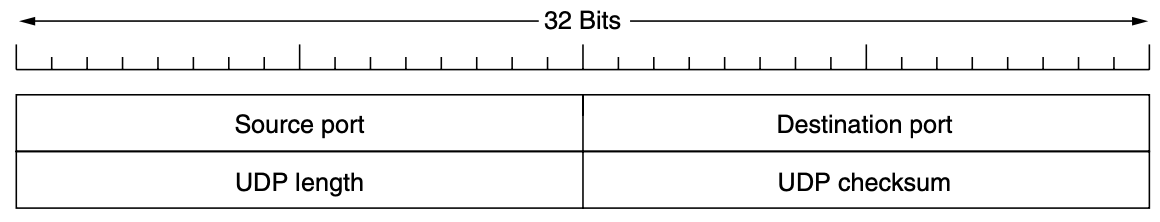
\includegraphics[width=1\linewidth]{figures/tcpip_refmodel/image6.png}
    \caption[Structure of the UDP Header]{Structure of the UDP Header. Source: \cite{Tanenbaum2010}.}
    \label{fig:UDPHeader}
\end{figure}

Figure \ref{fig:UDPHeader} displays the UDP header, which has a size of 8 bytes. It is considerably smaller than the TPC header, which has a size of 20 bytes.

The header includes the fields \textit{Source port} and \textit{Destination port} to identify the endpoints in the respective instance. When a packet arrives, the payload is passed to the application using the appropriate port number via the UDP protocol.

The \textit{UDP length} field indicates the length of the segment, including the header. The maximum length of data that can be transmitted via UDP is limited to 65,515 bytes due to the underlying Internet Protocol.

The last field of the header is a 16-bit \textit{UDP checksum}. This checksum is formed via the so-called IP pseudoheader, which contains the source and destination IP address, the protocol number from the IP header, and the \textit{UDP length} field of the UDP header.

Compared to TCP, UDP can achieve higher data transmission speeds due to its lower protocol overhead, ase the UDP header is only 8 bytes in size. Furthermore, UDP does not require an acknowledgement of the transport or other mechanisms used by TCP to provide a reliable connection. This makes it very efficient and reduces processing overhead.



\section{Linux-Kernel}
% TODO






\section{UDP communication with a Linux Operating System}
% TODO

\subsection{Socket Types}
% TODO


\subsubsection{UDP Sockets}
% TODO


\subsubsection{Raw Sockets}
% TODO


\subsubsection{Packet Sockets}
% TODO


\subsection{Sending and Receiving a Packet}
% TODO


\section{Tuning Options}

\subsection{Quality of Service} \label{background:tuning:qualityofservice}


% TODO